\documentclass[10pt,a4paper]{article}
% This file compiles fine with pdflatex,
% (here: TeX Live 2013/Frankfurt Institute for Advanced Sciences)
\usepackage[utf8]{inputenc}
\usepackage{hyperref}
\hypersetup{linktocpage}
\usepackage[american]{babel}
\usepackage{amsmath} % xrightarrow, ...
\usepackage{cite}
\usepackage{units} % nicefrac
\usepackage{datetime} % time and \date
\usepackage{caption}
\usepackage{subcaption} % subfigures
\usepackage{graphicx} % pictures
\usepackage{tabularx} % tables
\usepackage{a4wide} % more space on sheets
\usepackage{amssymb} % symbols
\usepackage{array} % tables
\usepackage{booktabs} % better tables
\usepackage{floatrow} % caption beside image
\usepackage[toc,page]{appendix}

\usepackage[usenames,dvipsnames]{color} % more colors

% highlighting
\usepackage{xcolor}
\newcommand{\highlight}[1]{%
  \colorbox{green!30}{$\displaystyle#1$}}
  
% TODO boxes
% Alternative dazu (gut fuer Seitenanmerkungen):
% http://tex.stackexchange.com/a/73418/49958
%\usepackage[draft,colorinlistoftodos]{todonotes}   % notes showed

% Bibliography
\bibliographystyle{ieeetr}

% Colors (only used by hyperref)
\usepackage{color}
\definecolor{darkblue}{rgb}{0,0,.6}
\definecolor{darkred}{rgb}{.1,0,0}
\definecolor{darkgreen}{rgb}{0,.5,0}

% Hyperref for PDF
\hypersetup{
    pdftitle={Master Physik bei Nicolini, Calc writeup},
    pdfauthor={Sven Köppel},
    pdfsubject={master},
    pdfkeywords={physik} {master} {uni} {frankfurt} {fias},
    colorlinks=true,        % test: stat gerahmten Links
    linkcolor=red,          % color of internal links
    citecolor=darkgreen,    % color of links to bibliography
    filecolor=darkred,      % color of file links
    urlcolor=cyan           % color of external links
}

\title{Modified GUP in Extra Dimensions}
\author{\href{https://itp.uni-frankfurt.de/~koeppel}{Sven Köppel} \\
\texttt{koeppel@fias.uni-frankfurt.de}}
\date{Generation date: \today, \currenttime}

\begin{document}
\maketitle

% shorthands for differentials, etc
\renewcommand{\d}{\mathrm{d}}
\newcommand{\dd}[2]{\frac{\mathrm{d} #1}{\mathrm{d} #2}}
\newcommand{\pp}[2]{\frac{\partial #1}{\partial #2}}
\newcommand{\dann}{$\rightarrow~$}
\newcommand{\CA}{ {\cal A}}
\newcommand{\C}[1]{ {\cal #1} }
\newcommand{\mn}{_{\mu\nu}}
\newcommand{\bv}[1]{ \mathbf{ #1 } } % bold vector

% colored symbols:
% http://tex.stackexchange.com/questions/85033/colored-symbols
\newcommand*{\mathcolor}{}
\def\mathcolor#1#{\mathcoloraux{#1}}
\newcommand*{\mathcoloraux}[3]{%
  \protect\leavevmode
  \begingroup
    \color#1{#2}#3%
  \endgroup
}
% In Text: $a\textcolor{red}{\ast}b$
% In Math: $a\mathcolor{red}{\ast}b$
\newcommand{\redmin}{\mathcolor{red}{-}}
\newcommand{\redplus}{\mathcolor{red}{+}}
\newcommand{\pn}{\mathcolor{OliveGreen}{+ n}}
\newcommand{\n}{ {\mathcolor{OliveGreen}{n}} }

\begin{abstract}
This document subsumes calculations done based on the
paper \textit{Self-Completeness and the Generalized
Uncertainty Principle in Extra Dimensions} calculated by
Maximiliano Isi and Marco Knipfer \cite{work}. Their use of the GUP
in Large Extra Dimensions (LXDs) as proposed by Achim
Kempf 1995 allows non-convergent (aka Schwarzschild-Tangherlini like)
metrics at the origin.

Achim Kempf provided the mathematical framework for generic
GUP modifications \cite{kempf1995}. It is easy to choose one which features
regular solutions for any number of dimensions, but Marcos
integral solving approach (Schwinger Operator representation and identification as higher dimensional Gaussian integral) fails for that Ansatz. In this
document I will present another approach.

The issue was presented by Marco in Journal Club at 14-06-2014
and by Sven at 18-06-2014.

\hfill\textit{Internal working title:} \textsc{Calc17}
\end{abstract}


\tableofcontents

%\listoftodos

\newpage

%%%%%%%%%%%%% BEGIN OF CONTENT %%%%%%%%%%%%%%
\section{Framework}
This document follows the reasoning of the 2013 JHEP paper \cite{isi2013}. Skip section \ref{sec:intro1} if you are familiar with the notation of the work in progress \cite{work}.

\subsection{No extra dimensions} \label{sec:intro1}
I copy the notational introduction by Maximiliano from \cite{work} here. In $N+1=3+1$ space-time dimensions, we consider the GUP as modification of the canonical commutation relations ($p=|\bv p|$):
%
\begin{equation}
[x^i, p_j] = i \delta^i_j (1 + \beta p^2)
\end{equation}
%
Kempf \cite{kempf1995} showed how this results in a modified momentum integration measure,
\begin{equation} \label{eq:GUP1}
\int \frac{\d^3 p}{1 + \beta p^2} | p \rangle\langle p | = 1,
\end{equation}
which is used to determine the modified Einstein equations for with the momentum representation of the Dirac delta distribution:
%
\begin{align}
R\mn &= \frac 12 g\mn R = 8\pi G \C T\mn \\
\C T\mn &= \C A^{-2}(\square) T\mn \\
\C A^{-2}(\square) \delta(x) &= (2\pi)^{-3}
    \int \frac{\d^3 p}{1 + \beta p^2}  e^{i \bv x \cdot \bv p}
\end{align}
%
Our investigations work on static spherically symmetric sources $T_0^0 = M \delta(x)$ that lead to the well-known Einstein(-Tangherlini) modified metric. For convenience, we choose to sum up all non-local effects in the mass, that is,
%
\begin{equation}
\C M \delta(x) = M \C A^{-2}(\square) \delta(x),
\end{equation}
%
and except the new curly mass symbol $\C M$, the metric looks exactly like the $N+1$ dimensional Einstein(-Tangherlini) metric.

\subsection{Extradimensions}
With the presence of $n$ large extra dimensions, $N+1 = 4+n$ total space-time dimensions, Kempf proposes \cite{kempf1995}
%
\begin{equation}
\int \frac{\d^N p}{1 + \beta p^2} |p\rangle\langle p| = 1.
\end{equation}
%
It is easy to see that the powers of $p$ in the denominator must be increased for extra dimensions, for example by taking the series expansion of $1/f(p)$ at $p\to\infty$ (which corresponds with $\beta \to 0$):
%
\begin{equation} \label{eq:series-example}
\frac{1}{1 + \beta p^2} \approx \frac{1}{\beta p^2} 
- \C O\left( \frac{1}{\beta^2 p^4} \right)
% + \frac{1}{\beta^3 p^6}
\end{equation}
%
Only in the ordinary $N=4$ case, after radial composition of the integral \eqref{eq:GUP1}, the result looks like
\begin{equation}
\int \frac{ \d^3 p }{ 1 + \beta p^2}
\propto
\int \limits_{-\infty}^{\infty} \frac{ p^2~\d p }{ 1 + \beta p^2}
\stackrel{\text{\eqref{eq:series-example}}}{\approx}
\int \limits_{-\infty}^{\infty} \frac{\d p}{\beta}.
\end{equation}
%
The simplest possible extension of this approach is a modification of the GUP in $N+1$ dimensions
\begin{equation} \label{eq:improvedGUP}
[x^i, p_j] = i \delta^i_j (1 + L_n^{N-2} |\bv p|^{N-2})
\end{equation}
with the reduced planck scale in $n$ extradimensions $L_n$ and $\sqrt{\beta} = L_0$ the conventional Planck scale (in further equations, I will suppress the index of $L$ for readibility).

Defacto, the choice of arbitary GUPs was also handled in \cite{kempf1995}, Section 6.1. 

\section{Solving the energy density integral} \label{sec:content}
We now proceed to compute the line element
%
\begin{equation} \label{eq:start}
\C T_0^0 = M \frac{1}{(2\pi)^N} \int
\frac{\d^N p ~ e^{i \bv x \cdot \bv p}}{1 + L^{N-2} |\bv p|^{N-2}}
\end{equation}
%
My method does not make use of the Schwinger operator representation used in earlier papers, but residue theorem and Jordan's lemma to solve the integral \eqref{eq:start}. To apply them, I reduce the $N$-dimensional Fourier transformation to an effective one dimensional one.

Let's identify the integral to be solved with $\C I$ and the kernel with $V(\bv p)$:
\begin{equation}
\C T_0^0 = M \frac{1}{(2\pi)^N} \C I,
\quad 
\C I = \int V(\bv p)~e^{i\bv x \cdot \bv p} \d^N p,
\end{equation}
Using dimensionless coordinates $q = pL$ we write
\begin{equation}\label{eq:Vn}
V(p) = \frac{1}{1+L_p^{n+2} p^{n+2}} = \frac 1{1 + q^{n+2}}
\end{equation}
Using \eqref{eq:fourierNto1} from the appendix, we can integrate out all angles, resulting in
\begin{subequations}
\begin{align}
\label{eq:I1}
\C I &=
\underbrace{\frac{1}{(2\pi)^{3+n}}}_{\text{inv Four suppr.}}
 \frac{2\pi i}r \int_{-\infty}^\infty
\d p~
p^{1+n}
\left(
\frac{1}{1 + q^{n+2}} \Theta(q)
+ (-1)^n
\frac{1}{1 + (-q)^{n+2}} \Theta(-q)
\right)
~e^{ipr} \\
&=  \frac{2\pi i }{zL} \int_{-\infty}^\infty
\d q~
\frac{q^{1+n}}{L^{1+n}}
\left(
\frac{1}{1 + q^{n+2}} \Theta(q)
+ (-1)^n
\frac{1}{1 + (-q)^{n+2}} \Theta(-q)
\right)
~e^{iqz}
\label{eq:I2}
\end{align}
\end{subequations}
where the dimensionless $z=r/L$ is determined by requiring $e^{ipr} = e^{iqz}$. From \eqref{eq:I1} to \eqref{eq:I2} we note that the dimensionless calculation requires a global $\frac 1{L^{2+n}}$ scaling.

We now plan to solve \eqref{eq:I2} by cauchy theorem.

\subsection{The poles}
Consider the poles of \eqref{eq:Vn}. They are given by
\begin{equation} \label{eq:poles}
1 + q^{n+2} = 0
\quad\Leftrightarrow\quad
q = (-1)^{\frac 1{n+2}}
=\exp\left\{
\frac{i\pi + 2\pi i k}{n+2}
\right\}
\quad
\forall k\in \mathbb{N}_0
\end{equation}
There are $n+2$ unique poles, given e.g. by $k\in\{0,1,\dots,n,n+1\}$.

The integration contour is determined by requiring
\begin{equation} \label{eq:contour}
\lim_{p\to \pm i\infty} e^{ipz} = 0
~\Rightarrow~
e^{i(+i\infty)(+\#)} = e^{-i \infty \#} = 0
~\Rightarrow~
p\to i\infty
\end{equation}
as $z=|\bv z|$ is positive semi-definite. Therefore, only $\frac{n+2}{2}$ poles are taken into account.

One can check that no poles are on the real axis. For such poles,
\begin{subequations}
\begin{equation}
\operatorname{Im}(q)=0
\Leftrightarrow
\sin \left(\frac{\pi + 2\pi k}{n+2}\right)=0
\Leftrightarrow
\frac{1 + 2 k}{n+2} = 1 + j
\end{equation}
must hold in the domain of integral $k,j\in \mathbb{Z}_0$ for a given (integral) dimension $n$. The only solution is $q=-1$ which is not visible due to the $\Theta(q)$ in \eqref{eq:I2}.
On the other hand, for some $n$, there are poles on the imaginary axis:
\begin{equation}
\operatorname{Re}(q) = 0
\Leftrightarrow
\cos \left(\frac{\pi + 2\pi k}{n+2}\right)=0
\Leftrightarrow
\frac{1 + 2k}{n+2} = \frac 1 2 + j.
\end{equation}
\end{subequations}
is solved e.g. for $n=0,4,8$ and some $k, j$ (see Appendix \ref{appendix:fourier1} why that could be problematic).

\subsection{Performing Residue summation}
Factorizing the poles \eqref{eq:poles} in the integral \eqref{eq:I2}, suppressing prefactors, gives
\begin{equation}
\C I \propto \int
\d q ~q^{1+n} ~e^{iqz}
\left(
\frac{\Theta(q)}{
\prod \limits_{k=0}^{n+1} 
e^{\frac{i\pi + 2\pi i k}{2+n}} - q
}
+
\frac{(-1)^n \Theta(-q)}{
\prod \limits_{k=0}^{n+1} 
e^{\frac{i\pi + 2\pi i k}{2+n}} + q
}
\right)
\end{equation}

Actually, for all $n$,
%
\begin{equation} \label{eq:realRes}
\mathop{Res}_{q_0}
\frac{q^{1+n}}{1 + q^{n+2}}
:= r_0 \in \mathbb{Q}
\quad \forall q_0 \in
\{ q: q^{n+2} + 1 = 0 \},
\end{equation}
%
that is, the complex phases in the fourier coefficient $e^{iqz}$ survive in the residues except the very special situation $n=0$ where $q_0=\pm i$. Due to the symmetry of the poles (by construction), the complex phases of each two residues for poles $q_0=(-1)^\alpha$ and $\bar q_0=(-1)^{1-\alpha}$ kill each other: With the rational number $r_0$ as defined in \eqref{eq:realRes},
\begin{equation}
r_0 e^{i q_0 z} + r_0 e^{i \bar q_0 z}
= 2 r_0 e^{-z \sin(\pi \alpha)}
\cos\left( z \cos(\pi \alpha) \right).
\end{equation}

For the full results of the energy density, see table \ref{table:results}. Note that in the $n=0$ case, the result reduces to the well-known result from \cite{isi2013}. See \ref{fig:results-plot} for a plot of the energy densities.

\subsection{Mass and Metric behaviour}
Table \ref{table:results} motivates for a lookout about the black hole properties induced by the energy densities. For convenience I have sketched the metric coefficient in figure \ref{fig:g00},  given by integrating the mass $\C M(R) \propto \int _0^R \C T_0^0 r^{2+n} \d r$ (c.f. \cite{work} for notations).


\begin{table}[b!]
\renewcommand{\arraystretch}{1.7} % more line spacing
\begin{tabularx}{\textwidth}{ll}
\firsthline
$n$ & $\C I \propto \C T_0^0$ \\
\hline
0 & $-4/z \pi ^2 e^{-z} $ \\
1 & $-\frac{8}{3z} \pi ^2 e^{-\frac{\sqrt{3} z}{2}} \cos \left(\frac{z}{2}\right)$ \\
2 & $-2/z \pi ^2 e^{-\frac{z}{\sqrt{2}}} \cos \left(\frac{z}{\sqrt{2}}\right)$ \\
3 & $-\frac{8}{5z} \pi ^2 e^{-\frac{1}{2} \sqrt{\frac{1}{2} \left(5-\sqrt{5}\right)} z} \cos \left(\frac{1}{4}
   \left(1+\sqrt{5}\right) z\right)$ \\
4 & $-\frac{4}{3z} \pi ^2 e^{-z} \left(e^{z/2} \cos \left(\frac{\sqrt{3} z}{2}\right)+1\right)$ \\
5 & $\frac{8}{7z} \pi ^2 \left(-e^{-z \sin \left(\frac{\pi }{7}\right)} \cos \left(z \cos \left(\frac{\pi
   }{7}\right)\right)-e^{-z \cos \left(\frac{\pi }{14}\right)} \cos \left(z \sin \left(\frac{\pi
   }{14}\right)\right)\right)$ \\
6 & $\frac{\pi ^2}z \left(-e^{-z \sin \left(\frac{\pi }{8}\right)} \cos \left(z \cos \left(\frac{\pi
   }{8}\right)\right)-e^{-z \cos \left(\frac{\pi }{8}\right)} \cos \left(z \sin \left(\frac{\pi
   }{8}\right)\right)\right)$ \\
7 & $\frac{8}{9z} \pi ^2 \left(-e^{-\frac{\sqrt{3} z}{2}} \cos \left(\frac{z}{2}\right)-e^{-z \sin
   \left(\frac{\pi }{9}\right)} \cos \left(z \cos \left(\frac{\pi }{9}\right)\right)\right)$ \\
\hline
\end{tabularx}
\caption{Exact results of \eqref{eq:I2} in $n$ large extra dimensions (only missing the dimensionful $1/L^{2+n}$ scaling)} \label{table:results}
\end{table}

\begin{figure}
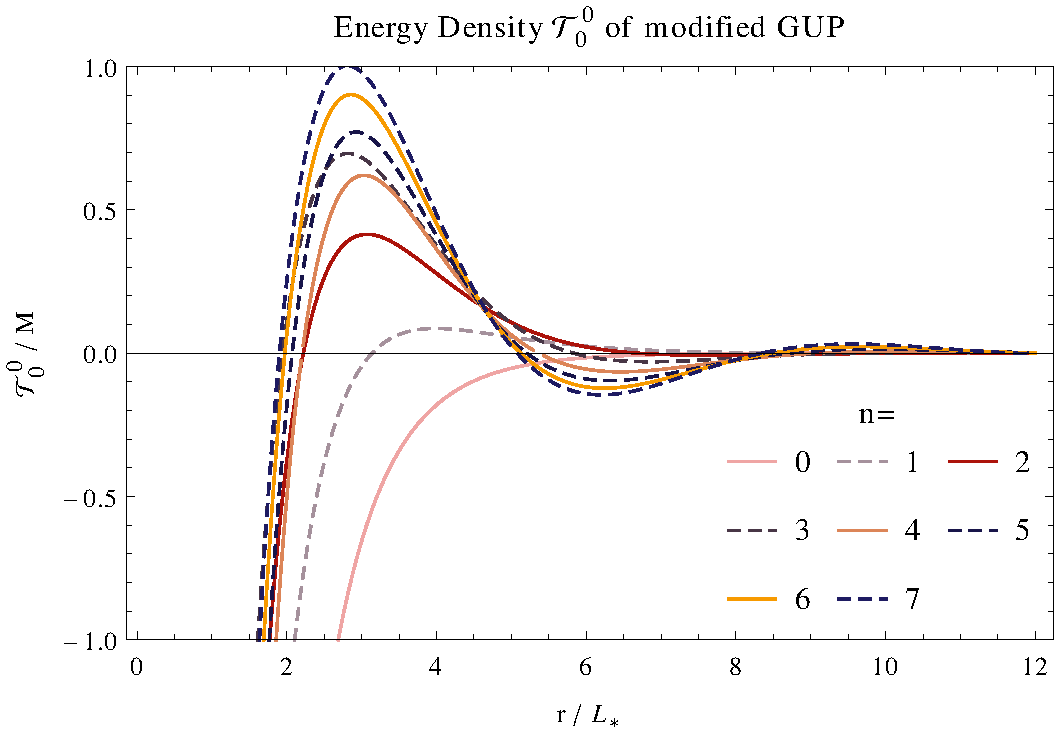
\includegraphics[width=0.8\textwidth]{plot/matter-density.pdf}
\caption{Plot of the functions in table \ref{table:results}.}\label{fig:results-plot}
\end{figure}

\begin{figure}
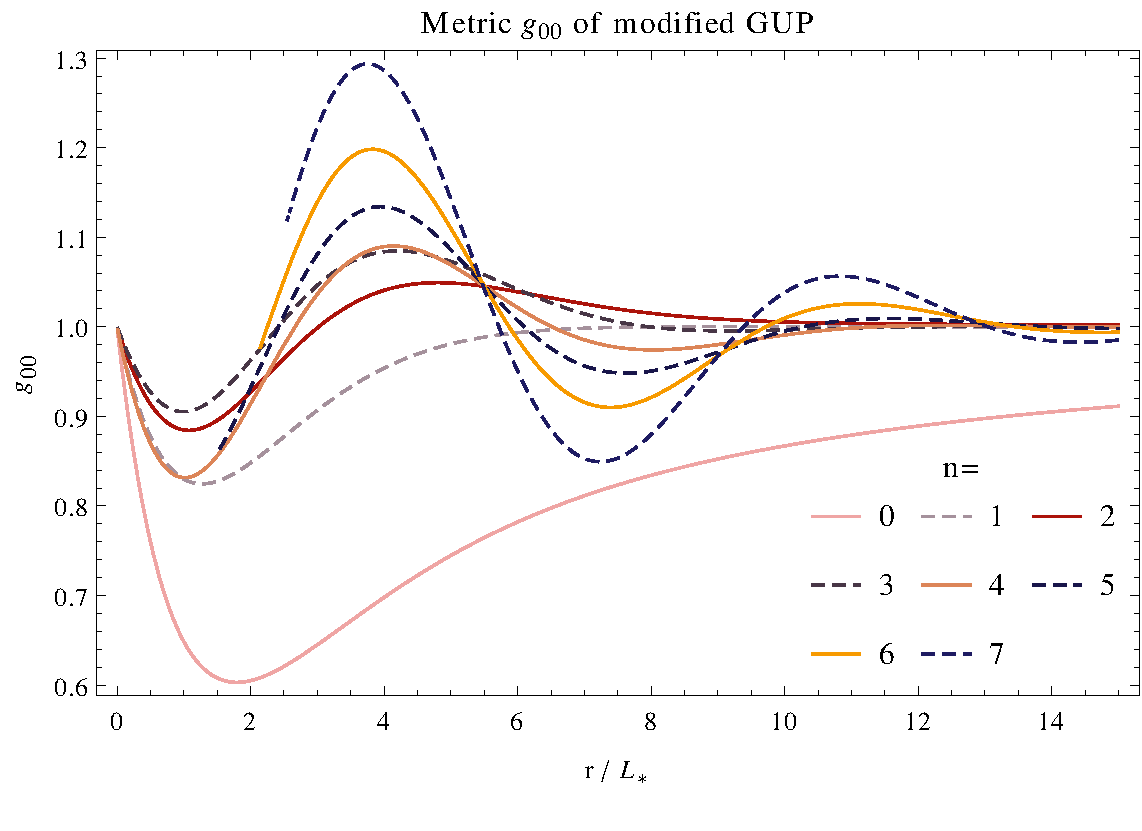
\includegraphics[width=0.8\textwidth]{plot/g00.pdf}
\caption{Plot of the line element of the modified GUP metrics in higher dimensions $n$.}\label{fig:g00}
\end{figure}



\newpage
\begin{appendices}
The following calculations retrace reducing higher dimensional Fourier transformations to one dimensional ones. While the 3d case (c.f. section \ref{appendix:fourier1}) is really well known, in literature I didn't found the derivation of the higher dimensional case (c.f. section \ref{appendix:fourierN}). Anyway, qualitatively the result is the same as in 3 dimensions and therefore the calculations are not that exciting but given for completeness.

\section{Review of the radial symmetric $d$-dimensional FT} \label{appendix:fourier}
Having the Fourier transformation $\C F_d$ in $d$ dimensions ($\bv x \in \mathbb R^d$) defined as
%
\begin{subequations}
\begin{align}
\C F_d\left\{ f \right\}(\bv p) &= \tilde f(\bv p) = \frac 1{(2\pi)^d} \int \d^d x~e^{-i\bv p \cdot \bv x} f(\bv x) \label{eq:Four1} \\
\C F^{-1}_d\left\{ \tilde f \right\}(\bv x) &= f(\bv x) =   \int d^d p~e^{+i \bv p \cdot \bv x} \tilde f(\bv p) \label{eq:Four2}
\end{align}
\end{subequations}
%
For shortness of notation, I will supress the leading $(2\pi)^d$ in the following equations.

The following calculations compute $\hat V = \C F\{V\}$, that is, going from position to momentum space. That is because I used them to extend \cite{NS2012}. Of course they also hold for the inverse, as used in section \ref{sec:content}.

\subsection{3d Fourier transformation} \label{appendix:fourier1}
We start the derivation in $d=3$ total spatial dimensions ($\vec r \in \mathbb R^3$). Let $V=V(r)$ with $r=|\vec r|$ be a radially symmetric potential. Then it's fourier transformation is given by:
%
\begin{subequations}
\begin{align}
\hat V(p) &= \int \d^3 r ~e^{-i \vec r \cdot \vec p}~ V(r) \\
&= \int_0^\infty \d r \int_0^\pi r^2 \sin \theta ~ \d \theta \int_0^{2\pi} \d \varphi~V(r)~e^{-i p r \cos \theta_2} \label{eq:f2}
\intertext{In line \eqref{eq:f2} we already wrote the scalar product with an inner angle $\theta_2$. We now substitute the radial angle $\theta$ (the $\theta$ which is part of $\vec r = (r,\theta,\varphi)$) integration with a $\cos \theta$ integration. This can be done because $\dd{\cos \theta}\theta = -\sin \theta$ and so $\int_0^\pi \sin \theta \d \theta = -\int_{-1}^1 \d \cos \theta = \int_{-1}^1 \d \cos \theta := \int_{-1}^1 \d x$. We now identify $\cos \theta := x$ with $\cos \theta_1$ because they share the same domain, actually $\theta,\theta_1 \in \{0,\pi\}$ (this is a standard procedure, one can also argue with rotating the coordinate systems. I think nobody doubts this substitution). We continue (naturally, $\int_0^{2\pi}\d \varphi = 2\pi$ was already integrated out in the next line):
}
&= 2\pi \int_{-1}^{+1} \d x \int_0^\infty \d r ~r^2 ~e^{-i r p x} V(r) \\
&= 2\pi \int_0^\infty r^2 ~  \d r ~ V(r) \left[ \frac{1}{-ipr} e^{-iprx} \right]_{-1}^{+1} \\
&= \frac{2\pi i}p \int_0^\infty r~\d r~V(r) \left\{ e^{-ipr} - e^{+ipr} \right\} \\
&= \frac{2\pi i}p \left\{ \int_0^\infty r~\d r~V(r) e^{-ipr} - \int_0^\infty r~\d r~V(r) e^{+ipr} \right\} \label{eq:f3}
\intertext{In line \eqref{eq:f3}, we splitted the integral, and we now make two recastings: At first, switching the integral borders, which inserts one \textcolor{red}{minus}: $\int_a^b = \redmin \int_b^a$ in \eqref{eq:f4}. Second, another substitution of the integration parameter $r:=\redmin r'$ and therefore $\d r = \redmin \d r'$. The two minus signs kill each other in \eqref{eq:f5}, so $r \d r = r' \d r'$. After substitution, we will call $r'$ again $r$, which is totally valid.
}
&= \frac{2\pi i}p \left\{ \int_0^\infty r~\d r~V(r) e^{-ipr} \redplus \int_{\infty}^0 r~\d r~V(r) e^{+ipr} \right\} \label{eq:f4} \\
&= \frac{2\pi i}p \left\{ \int_0^\infty r~\d r~V(r) e^{-ipr} \redplus \int_{\redmin \infty}^0 r'~\d r'~V(\redmin r') e^{\redmin i p r'} \right\}  \label{eq:f5} \\
&= \frac{2\pi i}p \int_{-\infty}^\infty r~\d r~ e^{-ipr}~
\left\{ V(r) \Theta(r) + V(-r) \Theta(-r) \right\} \label{eq:f6} \\
&= \frac{2\pi i}p \int_{-\infty}^\infty \d r~ \left\{ r V(|r|) \right\}~e^{-ipr} \label{eq:f7}
\end{align}
\end{subequations}
Basically \eqref{eq:f7} is our final result. The more extensive eq. \eqref{eq:f6} may be better to argue why I think the new {\it effective} one dimensional function (``kernel'') $v(r)\sim r~V(|r|)$ can still be treated as a holomorphic function when $\Theta$ is implemented as a smeared distribution. Discontinuities of $v(r)$ at $r=0$ may be discussed. If there are no poles at $r=0$, it should be always possible to let $V(-r)$ and $V(r)$ blend into each other in a continous way.

Whats about the real and complex parts of this fourier transformation? By construction, $V(|r|)$ is an even function (definition: $f(x)=f(-x)$ is even, $-f(x)=f(-x)$ is odd). Therefore $r~V(|r|)$ is an odd function. By eulers formula $e^{i\varphi} = \cos \varphi + i \sin \varphi$, one quickly finds that the Fourier Transform of an even function includes only (also even) $\cos$ terms and the complex part vanishes, while the FT of an odd function only contains $\sin$ terms and the real part vanishes. The integral in \eqref{eq:f7} is therefore ony complex, $\int \d r~rV(|r|)e^{-ipr} \in \mathbb{C} \setminus \mathbb{R}$. But the prefactor makes the final result in \eqref{eq:f7} completely real again. This can help as a quick check wether the computed result of the integral is correct.

The analytic continuation of the Heaviside function may be another issue. I think it can be again motivated by continuing the integral of a Dirac delta approximation like the Cauchy distribution. Anyway I always use the complex Heaviside function like $\Theta(z) = \Theta(\mathop{Re} z)$ which looks intrinsically non-holomorphic. Since there is no ordering relation $\leq_\mathbb{C}$ in the complex numbers, the theta is likely to behave differently on the complex plane. Anyway in three dimensions this approach is well known and works, so it should work in any number of dimensions.

\subsection{From 3 to (3+n) dimensions} \label{appendix:fourierN}
Consider the Fourier transformation in $d=3\pn$ dimensions. Following the same steps as in section \ref{appendix:fourier1}, we integrate out the angles of the measure (omitting the fourier kernel for shortness)
%
\begin{subequations}
\begin{align}
\int \d^d r &= \int_0^\infty \d r ~r^{d-1}
\int_0^{2\pi} \d \phi
\prod_{i=1}^{d-2} \int_0^\pi \d \theta_i \sin^i (\theta_i)
:= \int_0^\infty \d r ~\Omega_{d-1} r^{d-1} \\
&= \frac {\Omega_{d-1}}2 \underbrace{\int_0^\pi \d \theta_1 \sin(\theta_1)}_{=2} \int_0^\infty \d r ~r^{d-1}
\quad\quad
\text{with}
\quad
\Omega_{n+2} = 2 \frac{\pi^\frac{n+3}{2}}{\Gamma\left(\frac{n+3}{2}\right)}
\label{eq:df0b}
\end{align}
\end{subequations}
%
The $\theta_1$ integral in \eqref{eq:df0b} can only be evaluated to $\int \d \theta_1 \dots = 2$ if the integrand (which is ommitted in these equations) is not dependend of $\theta_1$. In our calculation, of course, this is not the case.

When doing the $\int_0^\infty \to \int_{-\infty}^\infty$ trick, an \emph{alternating minus} enters the effective fourier transformation kernel $v(r)$, taking account for the even/odd behaviour of the integrand. We end up with
%
\begin{equation}\label{eq:fourierNto1}
\hat V(p) = \frac {\Omega_{2\pn}}2  \frac{2\pi i}p
\int_{-\infty}^{\infty} \d r~r^{1\pn} \left( V(r) \Theta(r) + (-1)^{\n} V(-r) \Theta(-r) \right)
\end{equation}
%
Pay attention the toggling minus $(-1)^\n=(-1)^{2\pn}$, this does {\bf not} allow writing the effective integrand function $v(r)$ in a short way like $v(r) \neq r^{1\pn} V(|r|)$ as the naive extension of \eqref{eq:f7} could suggest. Why is it not $(-1)^{1\pn}$? Because when substituting $r\to\redmin r'$ and $\d r\to\redmin \d r'$,
\begin{equation}
r^{1\pn}\d r = (\redmin 1)^{1+n} (r')^{1+n} (\redmin1) \d r'
= (\redmin 1)^{\n} r'\d r'
\end{equation}
We end up with the nice and expected result that $v(r)$ is {\bf always odd} for all $n$, therefore $\forall n$:
\begin{subequations}
\begin{align}
\int \d r ~v(r) &\in \mathbb{C} \setminus \mathbb{R}
\\
\C F_{n+3}\left\{ V(|\vec r|) \right\} &\in  \mathbb{R}
\end{align}
\end{subequations}


\end{appendices}

\begin{thebibliography}{}
\bibitem{work}
  M.~Isi, M.~Knipfer, J.~Mureika and P.~Nicolini,
  ``Self-Completeness and the Generalized Uncertainty Principle in Extra Dimensions,'' \textit{in progress} (my latest copy: April 26, 2014).
  
\bibitem{kempf1995}
  A.~Kempf, G.~Mangano and R.~B.~Mann,
  ``Hilbert space representation of the minimal length uncertainty relation,''
  Phys.\ Rev.\ D {\bf 52} (1995) 1108
  [\href{http://arxiv.org/abs/hep-th/9412167}{hep-th/9412167}].

\bibitem{isi2013}
  M.~Isi, J.~Mureika and P.~Nicolini,
  ``Self-Completeness and the Generalized Uncertainty Principle,''
  JHEP {\bf 1311} (2013) 139
  [\href{http://arxiv.org/abs/arXiv:1310.8153}{arXiv:1310.8153 [hep-th]}].
  
  
\bibitem{NS2012}
  P.~Nicolini and E.~Spallucci,
  ``Holographic screens in ultraviolet self-complete quantum gravity,''
  Adv.\ High Energy Phys.\  {\bf 2014} (2014) 805684
  [\href{http://arxiv.org/abs/arXiv:1210.0015}{arXiv:1210.0015 [hep-th]}].


\end{thebibliography}

\end{document}
